% 8185: Quant Bhandari PS1

\documentclass[12pt]{article}
%\usepackage[T1]{fontenc}
%\usepackage{lipsum}
\renewcommand{\baselinestretch}{1.2} 
\usepackage{graphicx}
\usepackage{hyperref}
\hypersetup{
    colorlinks=true,
    urlcolor=blue,
    citecolor=blue
}
\usepackage[export]{adjustbox}
\usepackage{subcaption}
\usepackage{amsmath}
\usepackage{amssymb}
\usepackage{amsfonts}
\usepackage{geometry}
\setcounter{MaxMatrixCols}{20}
\geometry{a4paper,
 left=3cm,right=3cm,
 top=1.5cm, bottom=1.5cm}

\usepackage{natbib}
\bibliographystyle{apalike}


%\usepackage{natbib}
%\setcitestyle{authoryear,open={(},close={)}}
\graphicspath{ {../figs/} }

\begin{document}
%\thispagestyle{myheadings}
%\markright{Indian Statistical Institute, New Delhi\hfill }

\title{Econ 8185 (002): Quant PS2}
\author{Bipul Verma}
\date{\today}
\maketitle

%\tableofcontents{}
\abstract{This document calculates the Optimal Ramsey policies with and without state contingent debts.}

\vspace{8cm}

%\begin{center}
%\includegraphics[scale=0.4]{isi_logo.png}
%\end{center}
%\begin{center}
%\begin{Large}
%INDIAN STATISTICAL INSTITUTE, NEW-DELHI.
%\end{Large}
%\end{center}


\newpage

\section*{Model}

\textbf{Technology:}\\
\begin{align*}
y_t(s^t) = \theta(s_t) n_t(s^t).
\end{align*}
\textbf{Resource Constraint:}\\
\begin{align*}
y_t(s^t) = g_t(s^t) + c_t(s^t).
\end{align*}
\textbf{Utility:}\\
\begin{align*}
U(c, n) = u(c) - v(n)
\end{align*}
\textbf{Household Budget:}\\
\begin{align*}
c_t(s^t) + \sum_{s^{t+1}|s^t} P_{t+1}(s^{t+1}|s^t)b_{t+1}(s^{t+1}|s^t) = (1-\tau_t(s^t))\theta_t(s^t)n_t(s^t) + b_t(s_t|s^{t-1}).
\end{align*}
\textbf{Government Budget:}\\
\begin{align*}
g_t(s^t) =   \tau_t(s^t)\theta_t(s^t)  n_t(s^t) + \sum_{s_{t+1}} P_{t+1}(s_{t+1} | s^t) b_{t+1}(s_{t+1} | s^t) -
b_t(s_t | s^{t-1})
\end{align*}
\textbf{Shock Process:}\\
\begin{align*}
\ln(g_{t+1}) = (1-\rho_g)\mu_g + \rho_g \ln( g_t) + N(0, \sigma_g^2)\\
\ln(\theta_{t+1}) = (1-\rho_\theta)\mu_\theta + \rho_\theta \ln(\theta_t) + N(0, \sigma_\theta^2)
\end{align*}

\section{Computation Algorithm}
\subsection{With State Contingent Debt}
\begin{enumerate}
\item Guess $\Phi$.
\item Compute $\{c(s), n(s) \}$ for all $s$ for given $\Phi$ using the following equations:
\begin{align*}
& (1+\Phi)[u_c(c)\theta + u_n(n)] + \Phi[cu_{cc}(c)\theta + nu_{nn}(n)] =0 \\
& n = \frac{g + c}{\theta}
\end{align*}
\textit{Note that given the Markov structure of shocks, the above solves for policies for all $t\geq 1$ .} It is understood that $c$ and  are $g$ each functions of the Markov state $s$.
\item Compute $\{c_0(s_0, b_0), n_0(s_0, b_0) \}$  using:
\begin{align*}
& (1+\Phi) [u_c(c_0)\theta + u_n(n_0)] + \Phi[c_0 u_{cc}(c_0)\theta + n_0 u_{nn}(n_0)] - \Phi u_{cc}(c_0) b_0 \theta = 0 \\
& b_0 = 4 \theta_0 n_0 \\
& n_0 = \frac{g_0 + c_0}{\theta_0}.
\end{align*}
\item Evaluate the implementation constraint as follows:
\begin{align}\label{implementation}
& u_{c,0} b_0 = u_{c,0} c_0 + u_{n,0} n_0  + \beta \sum_{s} \Pi(s | s_0) sum(s)
\end{align}
where $sum(s)$ solves the following $S \times 1$ system of equations for $s \in \{1, 2, \dots, S \}$:
\begin{align*}
& sum(s) = u_{c}(s) c(s) + u_{n}(s) n(s)  + \beta \sum_{s'} \Pi(s' | s) sum(s').
\end{align*}
In matrix form the solution is given by:
\begin{align*}
\vec sum(s) = (I - \beta \Pi_s)^{-1}[\vec u_{c}(s) \vec c(s) + \vec u_{n}(s) \vec n(s)]
\end{align*}
where vector products are understood as element wise product.

\item If $LHS > RHS$ in \ref{implementation}, increase $\Phi$, if $LHS < RHS$ in \ref{implementation}, reduce $\Phi$.
\item Repeat the procedure to find $\Phi$ such that the implementation constraint binds.
\item \textit{Note:} Instead of updating $\Phi$ as in step $4, 5$, we can also solve for the root of \ref{implementation} to arrive at $\Phi$ such that \ref{implementation} binds.
\end{enumerate}

\subsection{Without State Contingent Debt}
In this case the problem can be reduced to solving the following two part bellman equation:\\
for $t\geq 1$ 
\begin{align*}
V(x_{-}, s_{-}) = \max_{c(s), n(s), x(s)} \sum_{s} \Pi(s|s_{-}) \{ U(c(s), n(s)) + \beta V(x(s), s) \}
\end{align*}
subject to 
\begin{align*}
& \frac{x_{-}U_c(s)}{\beta\sum \Pi(\tilde{s}|s_{-})U_c(\tilde{s}) } = U_c(s)c(s) + U_n(s)n(s) + x(s)  \\
& \theta(s) n(s) = c(s) + g(s) ; \; \; \; \; \forall s \in S
\end{align*}
for $t = 0$
\begin{align*}
& W(b_0, s_0) = \max_{c(s_0), n(s_0), x(s_0)}  U(c(s_0), n(s_0)) + \beta V(x(s_0), s_0)\\
\end{align*} 
subject to 
\begin{align*}
& U_c(s_0)b_0 = U_c(s_0)c(s_0) + U_n(s_0)n(s_0) + x(s_0)  \\
& \theta(s_0) n(s_0) = c(s_0) + g(s_0).
\end{align*}


\section{Portfolio of risk free bonds}
Following Angeletos(2002) %\cite{angeletos2002fiscal}
the complete markets Ramsey allocation can be implemented using bonds of maturity $1, 2, \dots, N$. In this case the households budget constraint is given by: 
\begin{align*}
c_t(s^t) + \sum_{n=1}^N q_t^{(n)}(s^t)b_t^{(n)}(s^t) = (1-\tau_t(s^t))\theta_t(s^t)n_t(s^t) + \sum_{n=1}^Nq_t^{(n-1)}(s^t)b_{t-1}^{(n)}(s^{t-1}); \, \, q_t^0 = 1.
\end{align*}
The price of bond is given by:
\begin{align*}
& q_t^{(n)}(s^t)= \beta \mathbb{E}_t[\frac{u_c(s^{t+1})}{u_c(s^t)}q_{t+1}^{(n-1)}(s^{t+1})] \\
& q_t^{(n)}(s^t) = \beta^n \mathbb{E}_t[\frac{u_c(s^{t+n})}{u_c(s^t)}].
\end{align*}
We can use the bond pricing equation to recursively substitute the demand for bonds. In addition we also substitute out taxes to express everything in terms of allocation. We thus get:
\begin{align*}
 \sum_{n=1}^Nq_t^{(n-1)}(s^t)b_{t-1}^{(n)}(s^{t-1})u_c(s^{t}) & = \underbrace{u_c(s^{t}) c_t(s^{t}) - u_\ell(s^{t}) n_t(s^{t})}_{x_t(s^t)} + \sum_{n=1}^N q_t^{(n)}(s^t)b_t^{(n)}(s^t) \\
 & = x_t(s^t) + \sum_{n=1}^N q_t^{(n)}(s^t)b_t^{(n)}(s^t)u_c(s^{t}).
\end{align*}
Now we substitute the bond price
\begin{align*}
& q_t^{(n)}(s^t)= \beta \mathbb{E}_t[\frac{u_c(s^{t+1})}{u_c(s^t)}q_{t+1}^{(n-1)}(s^{t+1})]
\end{align*}
in the previous equation to get:
\begin{align*}
\sum_{n=1}^Nq_t^{(n-1)}(s^t)b_{t-1}^{(n)}(s^{t-1})u_c(s^{t}) & = x_t(s^t) + \beta \sum_{n=1}^N \mathbb{E}_t[ q_{t+1}^{(n-1)}(s^{t+1})b_t^{(n)}(s^t)u_c(s^{t+1})]\\
& = x_t(s^t) + \beta  \mathbb{E}_t[ x_{t+1}(s^{t+1}) + \beta \mathbb{E}_{t+1}\sum_{n=1}^N[q_{t+2}^{(n-1)}(s^{t+2})b_{t+1}^{(n)}(s^{t+1})u_c(s^{t+2})]] \\
& = \sum_{j=0}^\infty  \sum_{s^{t+j}|s^t} \beta^j\pi_t(s^{t+j}|s^t)  x_{t+j}(s^{t+j})\\
& = \sum_{j=0}^\infty  \sum_{s^{t+j}|s^t} \beta^j \pi_t(s^{t+j}|s^t) [u_c(s^{t+j}) c_t(s^{t+j}) - u_\ell(s^{t+j}) n_t(s^{t+j})] \\
& = sum(s^{t})\\
& = u_c(s^{t}) c_t(s^{t}) - u_\ell(s^{t}) n_t(s^{t}) + \beta \sum_{s^{t+1}|s^t} \pi_t(s^{t+j}|s^t) sum(s^{t+1}).
\end{align*}


For Markov shock structure these simplifies to:
\begin{align*}
q^{(j)}(s) & = \beta \sum_{s'|s} \pi(s'|s) q^{(j-1)}(s') \frac{u_c(s')}{u_c(s)}\\
\sum_{n=1}^Nq^{(n-1)}(s)b_{-1}^{(n)}(s^{-1})u_c(s) & =  u_{c}(s) c(s) + u_{n}(s) n(s)  + \beta \sum_{s'} \Pi(s' | s) sum(s') \\
 & = \frac{sum(s)}{u_c(s)}
\end{align*}

For $N=S$, we have $N$ equations in $N$ variables which can be solved to get the portfolio of bonds of different maturity. Note that the system of equations in matrix form can be written as:
\begin{align*}
\mathbf{Q}\mathbf{b} = \mathbf{Z}.
\end{align*}
\textbf{Result:} We find that optimal portfolio of bonds involves sale and purchase of bonds in large quantities (in orders of magnitude of the gdp). This mirrors the findings in Buera-Nicolini-Pablo(2004). The interpretation is that since interest rates (bond prices) are closely correlated government has to take large asset positions in order to diversify risk.
%sum(s^{t+1}) & = \sum_{j=0}^\infty  \sum_{s^{(t+1)+j}|s^{t+1}} \beta^j \pi_{t+1}(s^{(t+1)+j}|s^{t+1})  [u_c(s^{(t+1)+j}) c_{t+1}(s^{(t+1)+j}) - u_\ell(s^{(t+1)+j}) n_{t+1}(s^{(t+1)+j})]

%%--------REFERENCES---------------%%
% https://python-advanced.quantecon.org/opt_tax_recur.html#equation-tss-techr-opt-tax

\section{Simulations}
\subsection*{Simulating Ramsey Policies with State contingent debt}
\begin{figure}[h]
    \centering
    \begin{minipage}{0.45\textwidth}
        \centering
        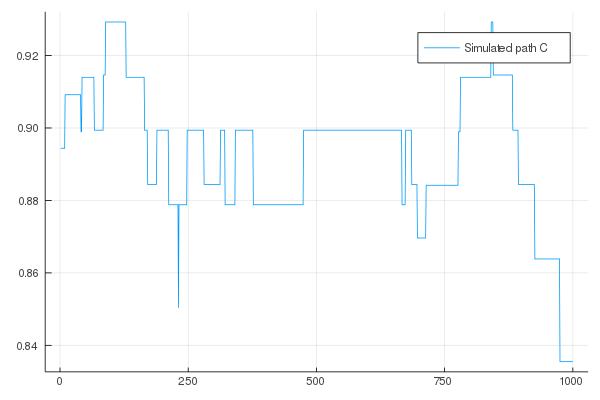
\includegraphics[width=1.2\textwidth]{ramsey_C.png} % first figure itself
        \caption{Consumption Policy Function}
    \end{minipage}\hfill
    \begin{minipage}{0.45\textwidth}
        \centering
        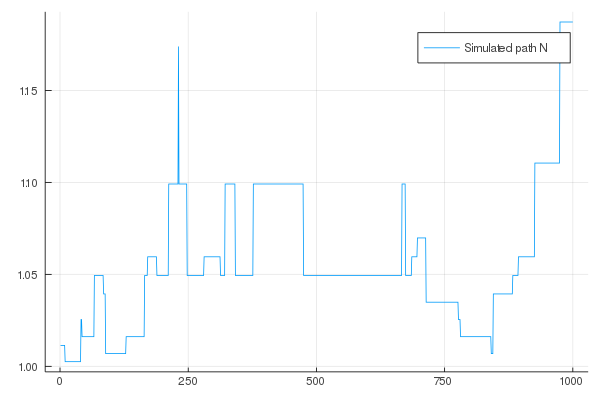
\includegraphics[width=1.2\textwidth]{ramsey_N.png} % second figure itself
        \caption{Labor Policy function}
    \end{minipage}
\end{figure}

\begin{figure}[h]
    \centering
    \begin{minipage}{0.45\textwidth}
        \centering
        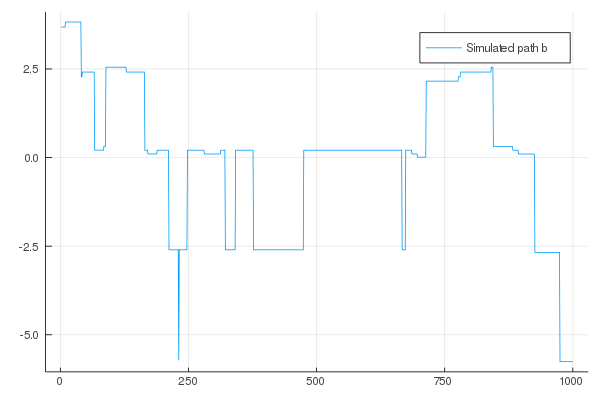
\includegraphics[width=1.2\textwidth]{ramsey_B.png} % first figure itself
        \caption{Bonds}
    \end{minipage}\hfill
    \begin{minipage}{0.45\textwidth}
        \centering
        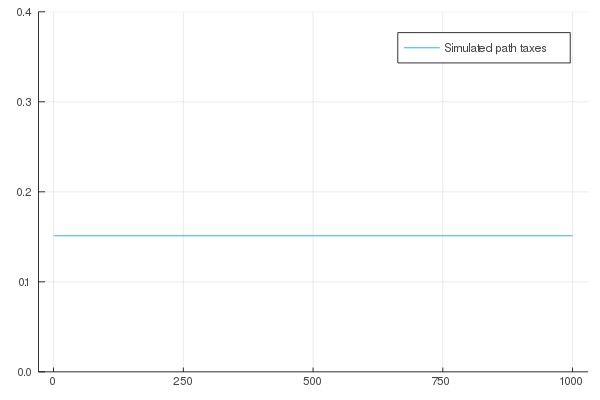
\includegraphics[width=1.2\textwidth]{ramsey_Tau.png} % second figure itself
        \caption{Taxes on labor}
    \end{minipage}
\end{figure}
\subsection*{Simple Example}
In order to verify our code we ran the model with the parameters in \href{https://python-advanced.quantecon.org/opt_tax_recur.html}{QuantEcon}. For this case we work with the following:
\begin{align*}
u(c,n) = {\frac{c^{1-\sigma}}{1-\sigma}} - {\frac{n^{1+\gamma}}{1+\gamma}},
\end{align*}
and set $\gamma = \sigma = 2$, and $\beta = 0.9$. We think of these 6 states as corresponding to $s=1,2,3,4,5,6$. The transition matrix is:
\begin{align*}
\begin{split}
\Pi = \left(\begin{matrix}0 & 1 & 0 & 0   & 0   & 0\\
                          0 & 0 & 1 & 0   & 0   & 0\\
                          0 & 0 & 0 & 0.5 & 0.5 & 0\\
                          0 & 0 & 0 & 0   & 0   & 1\\
                          0 & 0 & 0 & 0   & 0   & 1\\
                          0 & 0 & 0 & 0   & 0   & 1\end{matrix}\right)
\end{split}
\end{align*}
Government expenditures at each state are:
\begin{align*}
\begin{split}
g = \left(\begin{matrix} 0.1\\0.1\\0.1\\0.1\\0.2\\0.1 \end{matrix}\right)
\end{split}
\end{align*}
The results match exactly, confirming that our code for Ramsey is correct. Below are the figures from replication :
\begin{figure}[h]
    \centering
    \begin{minipage}{0.45\textwidth}
        \centering
        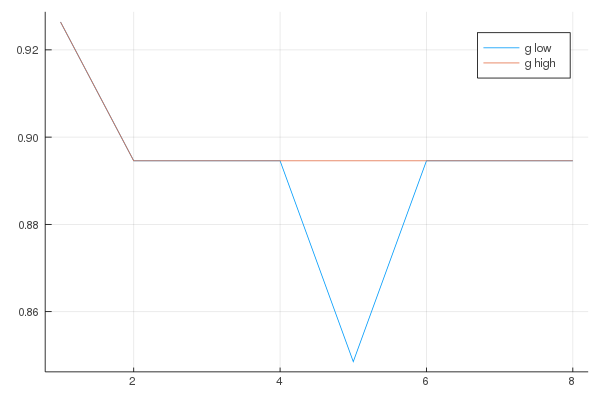
\includegraphics[width=1\textwidth]{QE_C.png} % first figure itself
        \caption{Consumption Policy Function}
    \end{minipage}\hfill
    \begin{minipage}{0.45\textwidth}
        \centering
        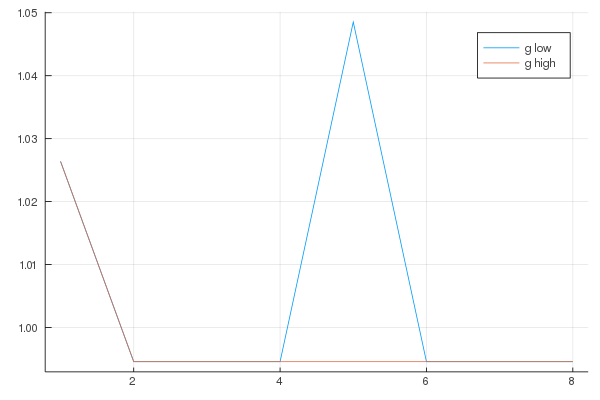
\includegraphics[width=1\textwidth]{QE_N.png} % second figure itself
        \caption{Labor Policy function}
    \end{minipage}
\end{figure}

\begin{figure}[h]
    \centering
    \begin{minipage}{0.45\textwidth}
        \centering
        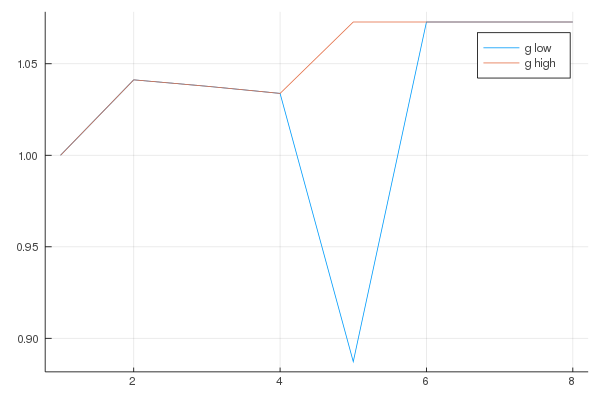
\includegraphics[width=1\textwidth]{QE_B.png} % first figure itself
        \caption{Bonds}
    \end{minipage}\hfill
    \begin{minipage}{0.45\textwidth}
        \centering
        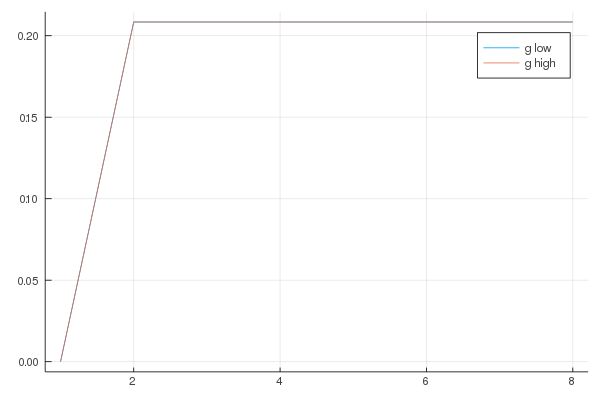
\includegraphics[width=1\textwidth]{QE_tau.png} % second figure itself
        \caption{Taxes on labor}
    \end{minipage}
\end{figure}





\newpage
\bibliography{ref}

\end{document}